\chapter{Analiti"cna izpeljava vplivov dinami"cne in stati"cne ekscentri"cnosti}

V tem poglavju bom sku"sal analiti"cno prikazati vpliv napak omenjenih ekscentri"cnosti, ki se pojavita zaradi neprimerne vgradnje te vrste enkoderja. Napaki razli"cno vplivati na izhode senzorja, zato ju lahko obravnamvam posami"cno. Preko analiti"cne izpeljave bomo spoznali kako se spreminja lokacija Hall-ove sonde glede na magnet ob pravilni monta"zi. Z vpeljavo dodane ekscentri"cnosti v model bomo videli, kako se trajektorija gibanja Hall-ove sonde glede na magnet spremeni. S poznavanjem lokacije Hall-ove sonde nad magnetom bomo lahko od"citali vrednost \Bz.


\section{Definicija koordinatnih sistemov}

Definirajmo kartezi"cni koordinatni sistem, ki ima v izhodi"scu postavljen radialno magnetiziran magnet. Na poljubno to"cko $S_{h0}(x_0,y_0)$, vendar ne v izhodi"s"ce postavimo Hall-ovo sondo. Na sliki \ref{fig:def_kks} je prikazan tak sistem. Hall-ova sonda je postavljena na abcisno os za la"zje razumevanje. Vrednost $y_0$ je lahko poljubna in kon"cna re"sitev izpeljave bo splo"sna za poljubno lokacijo Hall-ove sonde v za"cetni legi.

\begin{figure}[h!]
	\centering
	\begin{tikzpicture}
	\magnet {0} {0} {0}{$S_r(0, 0)$}{1};
	\hall {2.3}{0} {0};
	\end{tikzpicture}
	\caption{Definicija koordinatnega sistema z magnetom in Hall-ovo sondo}
	\label{fig:def_kks}
\end{figure}

Z rotacijo magneta za kot $\theta$, se lokacija Hall-ove sonde glede na magnet spremeni. Nova lokacija Hall-ove sonde glede na magnet je enaka, "ce namesto magnet, zarotiramo Hall-ovo sondo za kot $-\theta$ . Novo lokacjo Hall-ove sonde glede na magnet lahko zapi"semo z rotacijsko matriko.

\begin{equation}
\label{equ:rotacija_hall}
\begin{bmatrix} x\\y \end{bmatrix}=
\begin{bmatrix} \cos(-\theta)&-\sin(-\theta)\\\sin(-\theta)&\cos(-\theta) \end{bmatrix}
\begin{bmatrix} x_0\\y_0 \end{bmatrix}
\end{equation}

Argument rotacijske matrike je $-\theta$, pri "cemer vemo, da smo namesto magneta zarotirali Hall-ovo sondo v nasprotno smer. Z upo"stevanjem lihosti funkcije sinus in sodosti funkcije kosinus, se ena"cba \ref{equ:rotacija_hall} poenostavi v:
\begin{equation}
\label{equ:rotacija_hall_simplify}
\begin{bmatrix} x\\y \end{bmatrix}=
\begin{bmatrix} \cos(\theta)&\sin(\theta)\\-\sin(\theta)&\cos(\theta) \end{bmatrix}
\begin{bmatrix} x_0\\y_0 \end{bmatrix}
\end{equation}




\begin{figure}[h!]
%	\centering


    \begin{subfigure}[b]{0.5\textwidth}
	\centering
	
		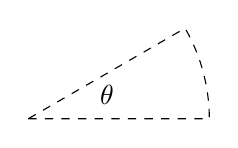
\begin{tikzpicture}
		[scale=1, every node/.style={scale=1}]
				\magnet {0} {0} {30}{}{1}
				\hall {2.3}{0} {0};
				\draw [dashed](0,0)--(2.3,0) arc (0:30:2.3)--(0,0);
				\node at(1,0.3){$\theta$};
		\end{tikzpicture}
	\caption{Zasukan magnet za kot $\mathrm{\theta}$}
	\label{subfig:zasuk_magnet}
\end{subfigure}
\begin{subfigure}[b]{0.5\textwidth}
	\centering
	
		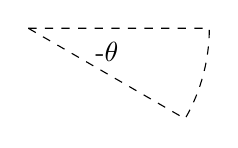
\begin{tikzpicture}[scale=1, every node/.style={scale=1}]		
				\magnet {0} {0} {0}{}{1}
				\hall {1.99}{-1.15} {-30};
				\draw [dashed](0,0)--(2.3,0) arc (0:-30:2.3)--(0,0);
				\node at(1,-0.3){-$\theta$};
		\end{tikzpicture}
	
	\caption{Zasukan senzor za kot $\mathrm{-\theta}$}
	\label{subfig:zasuk_hall}
\end{subfigure}

\caption{Sprememba lokacije glede na magnet ob rotaciji}
\label{fig:zasuk_magneta}

\end{figure}



\section{Izpeljava gibanja lokacije Hall-ove sonde na magnet pri dinami"cni ekscentri"cnosti}

Opazujmo sedaj sistem gibanja Hall-ove sonde glede na magnet ter dinami"cno ekscentri"cnost. Magnet je
 postavljen v izhodi"sce koordinatnega sistema $S_m(0,0)$. Sedaj magnet izmaknemo v novo lego $S_{m1}(\Delta
  x_d,\Delta y_d)$ (Slika \ref{fig:def_din_eks}). Os vrtenja je "se vedno postavljena v izhodi"s"ce
   koordinatnega sistema. Sredi"sce magneta $S_{m1}(\Delta x_d,\Delta y_d)$ tako tekom vrtenja okoli
    koordinatnega izhodi"sca opi"se kro"znico z radijem $\sqrt{\Delta x_d^2+\Delta y_d^2}$. V sistem sedaj
     dodajmo Hall-ovo sondo v njeno za"cetno lego glede na izhodi"sce $S_{h0}(x_0,y_0)$.




\begin{figure}[h!]
	\centering
	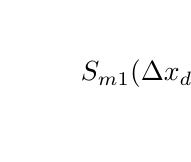
\begin{tikzpicture}
		\magnet {0.6} {0.3} {0}{$S_{m1}(\Delta x_d,\Delta y_d)$}{1};
		\draw [dashed]  (0,0) circle (0.67);
		\draw (0,0)--(0.6,0.3);
		\fill (0,0) circle [radius=1pt];
		\node at (0.35,-0.3){$S_0(0,0)$};
		\hall {2.3}{0} {0};
		\kks{3}
	\end{tikzpicture}
	\caption{Shema definicije dinami"cne ekscentri"cnosti vpliva na magnet}
	\label{fig:def_din_eks}
\end{figure}




Enako gibanje Hall-ove sonde na magnet lahko dose"zemo tudi z obrnjenim sistemom. Vrnimo magnet v izhodi"s"cno lego $S_m(0,0)$. Sedaj postavimo os vrtenja magneta v to"cko $(-\Delta x_d,-\Delta y_d)$. Hall-ovo sondo postavimo v to"cko $S_{h1}(x_0-\Delta x_d,y_0 - \Delta y_d).$



\begin{figure}[h!]
	\centering
	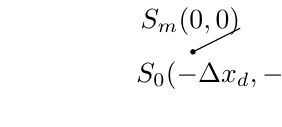
\begin{tikzpicture}
		\magnet {0} {0} {0}{$S_{m}(0,0)$}{1};
		\draw (0,0)--(-0.6,-0.3);
		\fill (-0.6,-0.3) circle [radius=1pt];
		\node at (0,-0.6){$S_0(-\Delta x_d,-\Delta y_d)$};
		\hall {1.7}{-0.3} {0};
		\kks{3}
	\end{tikzpicture}
	\caption{Shema definicije dinami"cne ekscentri"cnosti vpliva na Hall-ovo sondo}
	\label{fig:def_din_eks_na_stator}
\end{figure}

Sistema prikazana na slikah \ref{fig:def_din_eks} in \ref{fig:def_din_eks_na_stator}, se v za"cetnih legah ne razlikujeta. Sedaj zarotirajmo Hall-ovo sondo okoli osi vrtenja $S_0(-\Delta x_d,-\Delta y_d)$. Hall-ova sonda se giblje glede na magnet enako, kot "ce bi magnet zavrteli z dinami"cno ekscentri"cnostjo (Slika \ref{fig:def_din_eks}). Gibanje Hall-ove sonde na magnet je izra"zeno kot gibanje po kro"znici s sredi"s"cem v to"cki $(-\Delta x_d,-\Delta y_d)$.

\begin{figure}[h!]
	\centering
	\begin{tikzpicture}
		\magnet {0} {0} {0}{}{1};
		\draw [dotted]  (-0.6,-0.3) circle (2.3);
		\draw (0,0)--(-0.6,-0.3);
		\fill (-0.6,-0.3) circle [radius=1pt];
		\hall {1.39}{-1.45} {-30};
		\draw [dashed](-0.6,-0.3)--(1.7,-0.3) arc(0:-30:2.3)--(-0.6,-0.3);
		\node at(0.4,-0.6){$-\theta$};
		\kks{3}
	\end{tikzpicture}
	\caption{Potek Hall-ove sonde ob rotaciji glede na magnet ob dinami"cni ekscentri"cnosti}
	\label{fig:potek_sonde_din_eks}
\end{figure}

Potek Hall-ove sonde ob rotaciji z upo"stevanjem dinami"cne ekscentri"cnosti lahko zapi"semo kot (\ref{equ:rotacija_hall_simplify}) z dodatkom enosmerne komponente dinami"cne ekscentri"cnosti.

\begin{equation}
\label{equ:rotacija_hall_din}
\begin{bmatrix} x\\y \end{bmatrix}=
\begin{bmatrix} \cos(\theta)&\sin(\theta)\\-\sin(\theta)&\cos(\theta) \end{bmatrix}
\begin{bmatrix} x_0\\y_0 \end{bmatrix}
+
\begin{bmatrix} -\Delta x_d\\-\Delta y_d \end{bmatrix}
\end{equation}

V (\ref{equ:rotacija_hall_din}) lahko izrazimo - in izraz se poenostavi.

\begin{equation}
\label{equ:rotacija_hall_din_simplify}
\begin{bmatrix} x\\y \end{bmatrix}=
\begin{bmatrix} \cos(\theta)&-\sin(\theta)\\\sin(\theta)&\cos(\theta) \end{bmatrix}
\begin{bmatrix} x_0\\y_0 \end{bmatrix}
-
\begin{bmatrix} \Delta x_d\\\Delta y_d \end{bmatrix}
\end{equation}

\section{Izpeljava gibanja lokacije Hall-ove sonde na magnet pri stati"cni ekscentri"cnosti}


Postavimo sistem nazaj v izhodi"scno lego, brez ekscentri"cnosti. Tako sredisce magneta, kot os vrtenja postavimo v izhodi"sce. Hall-ova sonda je postavljena v to"cko $S_{h0}(x_0,y_0)$. Sedaj premaknimo Hall-ovo sondo za $(\Delta x_s, \Delta y_s)$, v novo to"cko $S_{h1}(x_0+\Delta x_s, y_0+\Delta y_s)$. Na sliki \ref{fig:def_sta_eks} je prikazana le stati"cna ekscentri"cnost v y-osi, vendar celotni razmislek velja za obe stati"cni ekscentri"cnosti enako.


\begin{figure}[h!]
	\centering
	\begin{tikzpicture}
	\magnet {0} {0} {0}{}{1};
	\hall {2.4}{-0.6} {0};
	\draw[<->,dotted] (0,0)--(0,-0.6);
	\draw[dotted] (2.3,-0.6)--(0,-0.6);
	\node at (0.4,-0.3){$\Delta y_s$};
	\end{tikzpicture}
	\caption{Shema definicije stati"cne ekscentri"cnosti}
	\label{fig:def_sta_eks}
\end{figure}

Po enakem razmi"sljanju kot v zgornjih poglavjih, sedaj zarotirajmo Hall-ovo sondo za kot \kol{-\theta} okoli izhodi"s"ca. Hall-ova sonda se giblje po kro"znici z radijem $\sqrt{(x_0+\Delta x_s)^2+(y_0+\Delta y_s)^2}$.


\begin{figure}[h!]
	\centering
	\begin{tikzpicture}
	\magnet {0} {0} {0}{}{1};
	\hall {1.69}{-1.67} {-30};
	\draw[<->,dotted] (0,0)--(-0.3,-0.52);
	\draw[dotted] (1.69,-1.67)--(-0.3,-0.52);
	\draw [dashed] (0,0) -- (2.377,0) arc(0:-30:2.377)--(0,0);
	\node at (0.8,-0.2) {\kol{-\theta}};
	\draw [dotted] (0,0)circle[radius=2.377];
    \draw [dotted, <->] (0,0)--(2.06,1.19);
    \node at (3.03,0.6){$\sqrt{(x_0+\Delta x_s)^2+(y_0+\Delta y_s)^2}$};
	
	\end{tikzpicture}
	\caption{Shema definicije stati"cne ekscentri"cnosti}
	\label{fig:def_sta_eks_stat}
\end{figure}












